\section{The Billing Framework architecture}\label{sec:the-code-derivation-pipeline}

As mentioned in section \addref rule-based systems require constant maintenance and rule updates.
Uncovered possible edge cases can appear even after system release.

As denoted in \addref one of the requirements for a rule-based system is extendability.
This does not only refer to the rules in the rule-base but also to the framework itself.
It must be straight forward to add new condition fields to the rule language.
This is why
I put great emphasis on extendability during the design of the Billing Framework
by making use of the pattern illustrated in figure \ref{fig:condition-triplet-pattern}.


\begin{figure}
    \centering
    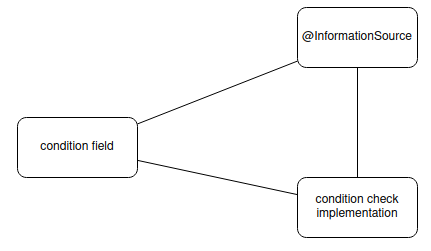
\includegraphics[width=0.75\linewidth]{./figures/condition-triplet-pattern}
    \caption{Geneic illustration of the triplet pattern}
    \label{fig:condition-triplet-pattern}
\end{figure}

Figure \addref and figure \addref display concrete instances of this pattern.


\begin{figure}
    \centering
    \begin{subfigure}[b]{0.45\linewidth}
        \centering
        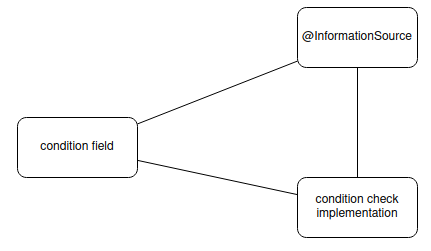
\includegraphics[width=\linewidth]{./figures/condition-triplet-pattern}
        \caption{Condition Triplet pattern instance 1}
        \label{fig:condition-triplet-pattern-instance-1}
    \end{subfigure}
    % Adjust or remove the space between figures as needed
    \hspace{5mm} % This adds a bit of horizontal space between the figures
    \begin{subfigure}[b]{0.45\linewidth}
        \centering
        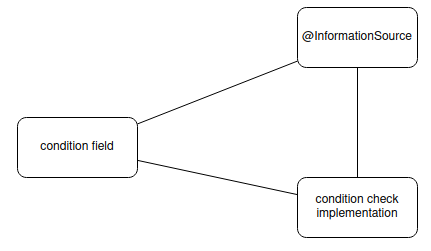
\includegraphics[width=\linewidth]{./figures/condition-triplet-pattern}
        \caption{Condition Triplet pattern instance 2}
        \label{fig:condition-triplet-pattern-instance-2}
    \end{subfigure}
    \label{fig:coffee}
\end{figure}



\subsection{Rule File Repository}
One component of the billing framework is the rule file repository.
This is the space where billing experts can work on the rule base, make changes and update existing rules.
To ensure semantic correctness, I use a schema validation library called Pydantic to validate rules loaded as python dictionaries.
It is extremely important that the system detects all issues at loading time.
Otherwise, the system will experience runtime issues due to invalid rules when deriving codes in production.

The rule loading procedure consists of the following steps:

A Python script is responsible for executing the following steps:
\begin{enumerate}
    \item Parse the rule file into a python dictionary
    \item Validate all dictionaries against the Pydantic rule schema.
    \item If all rules are valid, build a \code{RuleMsg} protobuf message from the validated dictionary
    \item Send all rules to the billing service using client-side gRPC streaming
    \item The billing service saves all received rule objects as a bulk transaction
\end{enumerate}

The rule file repository also stores the EBM and GOÄ datasets and provides client scripts for sending them to the billing service.
The billing service, requires both the rule and the catalogs to work properly.


\subsection{Billing server}
The billing server is a new microservice added to the microservice architecture of \AV.
It contains the full billing framework and implements the rule language specified in section \addref.

It exposes APIs for basic CRUD operations on billing positions, billing cases, code chains, code chain folder.
\code{applyCodeChainToBillingCase} merges all billing positions from the code chain into the current billing.

\lstinputlisting[
    language=protobuf2,
    style=protobuf,
    caption={BillingService gRPC service}
]{code/proto/architecture/billing-service.proto}


\lstinputlisting[
    language=protobuf2,
    style=protobuf,
    caption={BillingService gRPC service}
]{code/proto/architecture/catalog-service.proto}


\lstinputlisting[
    language=protobuf2,
    style=protobuf,
    caption={BillingService gRPC service}
]{code/proto/architecture/code-chains.proto}

The code derivation part is the most inte

\lstinputlisting[
    language=protobuf2,
    style=protobuf,
    caption={BillingService gRPC service}
]{code/proto/architecture/code-derivation.proto}

It exposes an API for basic CRUD operations on code chains and code chain folder.



\subsubsection{Rule Component}

\subsubsection{Rule Evaluation Input Fetcher}
A \code{RuleEvaluationInputFetcher} is a rule-type specific component responsible for fetching billing-relevant information from other services with the \AV microservice architecture.
They are auto-programmable components that hide fetching details from the rest of the system.
The term \"auto-programmable\" means that they configure themselves automatically upon rule loading.
This works as follows: The \code{Rule} entity class has as described before multiple condition fields.
The condition field names are equal to their corresponding condition keys in the rule language.
For each information source \todo{define information source}



It has access to the mi



